\chapter{Fundamentação Teórica}
\label{cap:fundamentacao}

\section{UML}
A UML (Unified Modeling Language) é uma linguagem gráfica que facilita a criação de softwares. Ela permite visualizar e detalhar os componentes de um sistema, como classes, objetos e suas interações, além de especificar o comportamento do sistema e documentar suas características. Tudo isso de forma padronizada e com o uso de diagramas, o que torna a comunicação entre os desenvolvedores mais fácil e eficiente \cite{uml:explicacao}. 
A referida tecnologia foi empregada para o desenho do fluxo dos microsserviços e da arquitetura, sendo escolhida por ser uma ferramenta de mercado para o desenho de arquiteturas de software e fluxos da aplicação.


\section{SQL}
A Linguagem de Consulta Estruturada (Structured Query Language - SQL) se configura como uma linguagem de programação padronizada para gerenciamento de dados em bancos de dados relacionais. Sua função primordial reside na manipulação, 
organização e recuperação de informações armazenadas nesses bancos, possibilitando aos usuários a consulta, inserção, atualização e exclusão de dados de forma eficiente e precisa \cite{sql:explicacao}.

A mencionada tecnologia foi utilizada na elaboração de \textit{procedures} no banco de dados do cliente e na criação das tabelas necessárias para os microsserviços, sendo selecionada em virtude dos bancos de dados serem relacionais.
\begin{figure}
    \centering
    \caption{Comandos sql}
    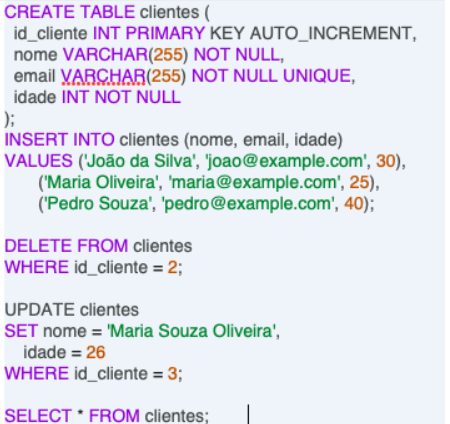
\includegraphics[width=0.5\textwidth]{arquivos/imagens/sql.png}
    \label{sql-comandos}
    \legend{Fonte: próprio autor }
\end{figure}

\section{SpringBoot}
O Spring Boot é um framework de software livre e open-source baseado na plataforma Java, projetado para facilitar e agilizar o desenvolvimento de aplicações web robustas e escaláveis. Sua principal característica reside na autoconfiguração, dispensando a necessidade de configurações manuais complexas e simplificando drasticamente o processo de criação de aplicações. Com o spring é possível criar aplicações Rest, Cloud, microsserviços entre outras arquiteturas \cite{spring:explicacao}.

A tecnologia em questão foi empregada no desenvolvimento dos microsserviços que compõem o projeto, mais especificamente: broker, onboarding, rotina de inativação de cliente e cadastro ou atualização de cliente. Tal escolha tecnológica decorreu da experiência dos profissionais seniores e plenos.

\section{SpringBootWeb}

Spring Web é um componente do Spring Framework que fornece suporte para a criação de aplicações web, incluindo recursos para desenvolvimento de controladores, gerenciamento de solicitações HTTP, manipulação de sessões e cookies, entre outros \cite{spring:web:explicacao}. Este componente foi empregado nos microsserviços para disponibilizar endpoints de comunicação via HTTP, sendo escolhido por ser um componente padrão dentro do ecossistema Spring.
\begin{figure}[h!]
    \centering
    \caption{Controlador Rest}
    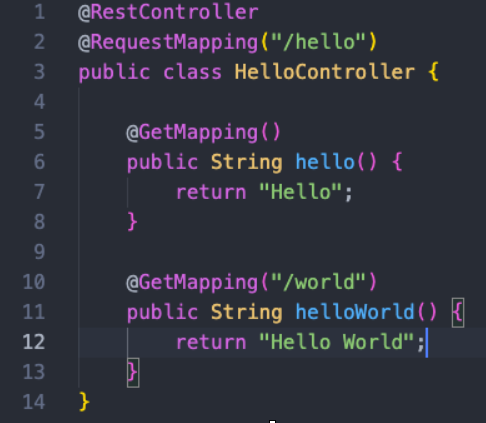
\includegraphics[width=0.5\textwidth]{arquivos/imagens/spring-web.png}
    \label{controlador rest}
    \legend{Fonte: próprio autor }
\end{figure}

\section{SpringWebFlux}

Spring WebFlux é um framework dentro do ecossistema Spring, desenvolvido para facilitar a construção de aplicativos reativos em Java. Ele oferece uma abordagem baseada em programação reativa para lidar com solicitações HTTP e interações assíncronas, permitindo que os desenvolvedores criem aplicativos altamente escaláveis e eficientes em termos de recursos \cite{spring:web:flux:explicacao}. 
Este framework foi empregado nos seguintes microsserviços: cadastro ou atualização de cliente, rotina de inativação de cliente e onboarding, visando efetuar requisições HTTP para o broker. A justificativa para sua escolha baseou-se na gestão mais avançada de requisições e na capacidade de realizar solicitações assíncronas.

\section{Flyway}

Flyway é uma ferramenta open-source específica para o ecossistema Java, que visa gerenciar versões dos bancos de dados relacionais a partir de arquivos SQL. A ferramenta exige que os arquivos sigam um padrão de nomeação, indicando o número da versão do script e o seu propósito \cite{flyway:explicacao}. 
Essa ferramenta foi utilizada nos microsserviços que requerem um banco de dados, para o controle das migrações do banco de dados em ambientes de homologação e produção.


\section{SWT}

A tecnologia SWT (Standard Widget Toolkit) é uma biblioteca gráfica destinada ao desenvolvimento de interfaces de usuário em Java. Desenvolvida pela Eclipse Foundation, é usada principalmente no ambiente de desenvolvimento Eclipse, mas pode ser empregada em outras aplicações java \cite{swt:explicacao}. 
A referida tecnologia foi utilizada para o desenvolvimento do ERP do cliente, pois era a única tecnologia disponível, em 2000, para a construção de aplicações desktop multiplataforma em Java.

\section{Metodologia}

O Kanban, que em japonês significa \enquote{cartão visual}, é um método de gestão de fluxo de trabalho que visa otimizar a entrega de valor através da visualização, limitação do trabalho em andamento e foco na melhoria contínua. Ele surgiu na Toyota na década de 1950 e se consolidou como uma das principais metodologias ágeis, utilizado em diversos contextos, desde o desenvolvimento de software até o gerenciamento de projetos e atividades pessoais, possuindo os seguintes princípios \cite{kanban:explicacao}:
\begin{enumerate}
    \item \textbf{Visualizar o Fluxo de Trabalho:} O Kanban se destaca por sua natureza visual, utilizando um quadro físico ou digital para representar as etapas do processo e o \textit{status} das tarefas. Essa representação gráfica facilita a compreensão do fluxo de trabalho, a identificação de gargalos e a comunicação entre os membros da equipe.
    
    \item \textbf{Limitar o Trabalho em Andamento (WIP):} O Kanban estabelece limites para o número de tarefas que podem estar em cada etapa do processo, impedindo o acúmulo excessivo de trabalho e promovendo o foco em atividades prioritárias. Essa limitação ajuda a reduzir o desperdício, aumentar a produtividade e garantir um fluxo de trabalho mais fluido.
    
    \item \textbf{Enfatizar a Entrega Contínua:} O Kanban incentiva a entrega frequente de valor ao cliente, seja mediante funcionalidades completas ou incrementos menores. Essa abordagem permite que os feedbacks sejam coletados e incorporados rapidamente, ajustando o curso do projeto conforme as necessidades do cliente.
    
    \item \textbf{Tornar Políticas Explícitas:} As regras e políticas que governam o fluxo de trabalho no Kanban são tornadas explícitas e visíveis para todos os envolvidos. Isso garante a transparência do processo, facilita a resolução de conflitos e promove a padronização das atividades.

    \item \textbf{Melhorar continuamente:} O Kanban incentiva a cultura da melhoria contínua, através da identificação e eliminação de desperdícios, otimização do fluxo de trabalho e experimentação de novas ideias. Essa mentalidade proativa leva a um processo em constante evolução e adaptação às necessidades do ambiente.
    
\end{enumerate}

Esse método foi selecionado para a gestão do projeto devido à sua capacidade de limitar o fluxo de trabalho em andamento, priorizar tarefas que geram valor para o cliente e proporcionar uma visualização clara do fluxo de trabalho tanto para os membros do projeto quanto para o cliente.
